\documentclass{article}
\usepackage[utf8]{inputenc}
\usepackage{listings}
\usepackage{color}
\usepackage{hyperref}
\usepackage{graphicx}
\usepackage[margin=1in]{geometry}  % Adjust margins
\usepackage{float}

\definecolor{codegreen}{rgb}{0,0.6,0}
\definecolor{codegray}{rgb}{0.5,0.5,0.5}
\definecolor{codepurple}{rgb}{0.58,0,0.82}

\lstdefinestyle{mystyle}{
    commentstyle=\color{codegreen},
    keywordstyle=\color{blue},
    stringstyle=\color{codepurple},
    basicstyle=\ttfamily\small,
    breakatwhitespace=false,         
    breaklines=true,                 
    keepspaces=true,                 
    showspaces=false,                
    showstringspaces=false,
    showtabs=false,                  
    tabsize=2
}

\lstset{style=mystyle}

\title{News Article Pipeline Implementation Report}
\author{Gokulakrishnan B \\ DA24M007}
\date{\today}

\begin{document}

\maketitle

\section{Introduction}
This report details the implementation of assignment 1 of DA5402 course, which aims to build an automated news article pipeline that scrapes, processes, and stores news articles from Google News. The system is designed with modularity in mind, comprising six distinct modules that handle different aspects of the pipeline.

\section{Database Setup}
First, we set up a PostgreSQL database to store our news articles and images, as it is highly scalable and used widely.

\subsection{Complete SQL Setup File}
The following SQL script (setup.sql) was used to create and configure the database:

\begin{lstlisting}[language=SQL]
-- Create the database
CREATE DATABASE news_db;

-- Connect to the database
\c news_db;

-- Create tables
CREATE TABLE news_articles (
    id SERIAL PRIMARY KEY,
    headline TEXT NOT NULL,
    article_url TEXT NOT NULL,
    publication_date TEXT NOT NULL
);

CREATE TABLE news_images (
    id SERIAL PRIMARY KEY,
    article_id INTEGER REFERENCES news_articles(id),
    thumbnail_url TEXT NOT NULL,
    image_data BYTEA NOT NULL
);

-- Create indexes for better query performance
CREATE INDEX idx_publication_date 
ON news_articles(publication_date);

CREATE INDEX idx_article_id 
ON news_images(article_id);

-- Grant necessary permissions
GRANT ALL PRIVILEGES ON DATABASE news_db TO postgres;
GRANT ALL PRIVILEGES ON ALL TABLES IN SCHEMA public TO postgres;
GRANT USAGE, SELECT ON ALL SEQUENCES IN SCHEMA public TO postgres;
\end{lstlisting}

\subsection{Database Schema}
The database consists of two main tables:

\begin{lstlisting}[language=SQL]
CREATE TABLE news_articles (
    id SERIAL PRIMARY KEY,
    headline TEXT NOT NULL,
    article_url TEXT NOT NULL,
    publication_date TEXT NOT NULL
);

CREATE TABLE news_images (
    id SERIAL PRIMARY KEY,
    article_id INTEGER REFERENCES news_articles(id),
    thumbnail_url TEXT NOT NULL,
    image_data BYTEA NOT NULL
);
\end{lstlisting}

\subsection{Database Connection}
The connection to PostgreSQL is handled using psycopg2:

\begin{lstlisting}[language=Python]
import psycopg2

def connect_db(config):
    return psycopg2.connect(
        dbname=config['database']['dbname'],
        user=config['database']['user'],
        password=config['database']['password'],
        host=config['database']['host'],
        port=config['database']['port']
    )
\end{lstlisting}

\section{Module Implementation}
 \\

\subsection{Module 1: Homepage Scraper}
This module serves as the entry point for the news scraping pipeline, covering the module 1 of the assignment. It handles the initial connection to Google News and manages HTTP requests with appropriate headers to avoid being blocked. The module is designed to be resilient against network errors and uses configurable user agents for flexibility.
To run this module, execute the following command:
\begin{lstlisting}[language=bash]
python module_1.py --config config.yaml
\end{lstlisting}

\begin{lstlisting}[language=Python]
class NewsHomeScraper:
    def __init__(self, config_path):
        with open(config_path, 'r') as f:
            self.config = yaml.safe_load(f)
        self.headers = {
            'User-Agent': self.config['scraper']['user_agent']
        }

    def scrape_homepage(self):
        try:
            response = requests.get(
                self.config['scraper']['base_url'], 
                headers=self.headers
            )
            response.raise_for_status()
            return response.text
        except Exception as e:
            print(f"Error scraping homepage: {e}")
            return None
\end{lstlisting}

\begin{figure}[H]
    \centering
    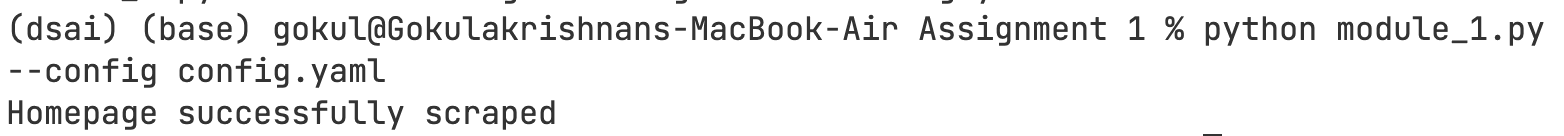
\includegraphics[width=\textwidth]{report/module_1 results.png}
    \caption{Results from Module 1 execution}
    \label{fig:module1-results}
\end{figure}

\\

\subsection{Module 2: Top Stories Link Extractor}
This module specializes in parsing the homepage HTML to locate the top stories section. It uses BeautifulSoup for the HTML parsing and implements intelligent link detection to find the most relevant news section. The module ensures we're always targeting the correct news feed even if the page structure changes slightly.
To run this module, execute the following command:
\begin{lstlisting}[language=bash]
python module_2.py --config config.yaml
\end{lstlisting}
\begin{lstlisting}[language=Python]
class TopStoriesScraper:
    def find_top_stories_link(self):
        soup = BeautifulSoup(self.homepage_content, 'html.parser')
        for a in soup.find_all('a', href=True):
            if 'top stories' in a.text.lower():
                return f"https://news.google.com{a['href']}"
        return None
\end{lstlisting}

\begin{figure}[H]
    \centering
    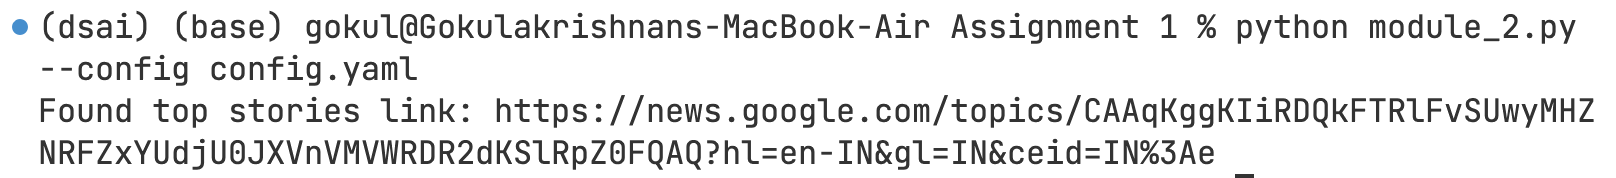
\includegraphics[width=\textwidth]{report/module_2 results.png}
    \caption{Results from Module 2 execution}
    \label{fig:module2-results}
\end{figure}

\\

\subsection{Module 3: Story Extractor}
The Story Extractor module is responsible for the detailed parsing of individual news articles. It handles various article formats and extracts key information like headlines, URLs, publication dates, and thumbnail images. The module includes retry logic for failed requests and implements rate limiting to avoid overwhelming the news server.
To run this module, execute the following command:
\begin{lstlisting}[language=bash]
python module_3.py --config config.yaml
\end{lstlisting}

\begin{lstlisting}[language=Python]
class StoryExtractor:
    def extract_stories(self, url):
        stories = []
        response = requests.get(url, headers=self.headers)
        soup = BeautifulSoup(response.text, 'html.parser')
        
        for article in soup.find_all('article'):
            story = self._extract_story_data(article)
            if story:
                stories.append(story)
        
        return stories
\end{lstlisting}

\begin{figure}[H]
    \centering
    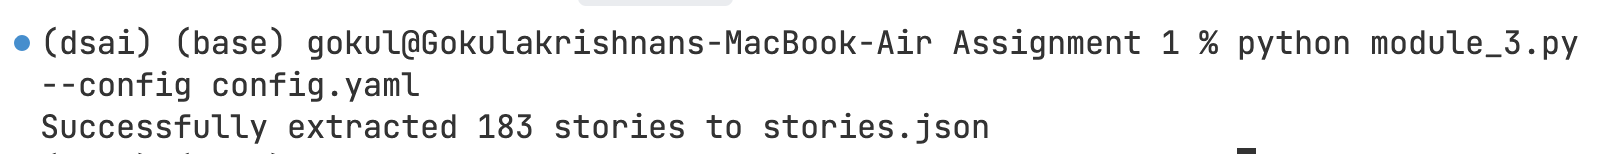
\includegraphics[width=\textwidth]{report/module_3 results_1.png}
    \caption{Results from Module 3 execution on terminal}
    \label{fig:module3-results-1}
\end{figure}

\begin{figure}[H]
    \centering
    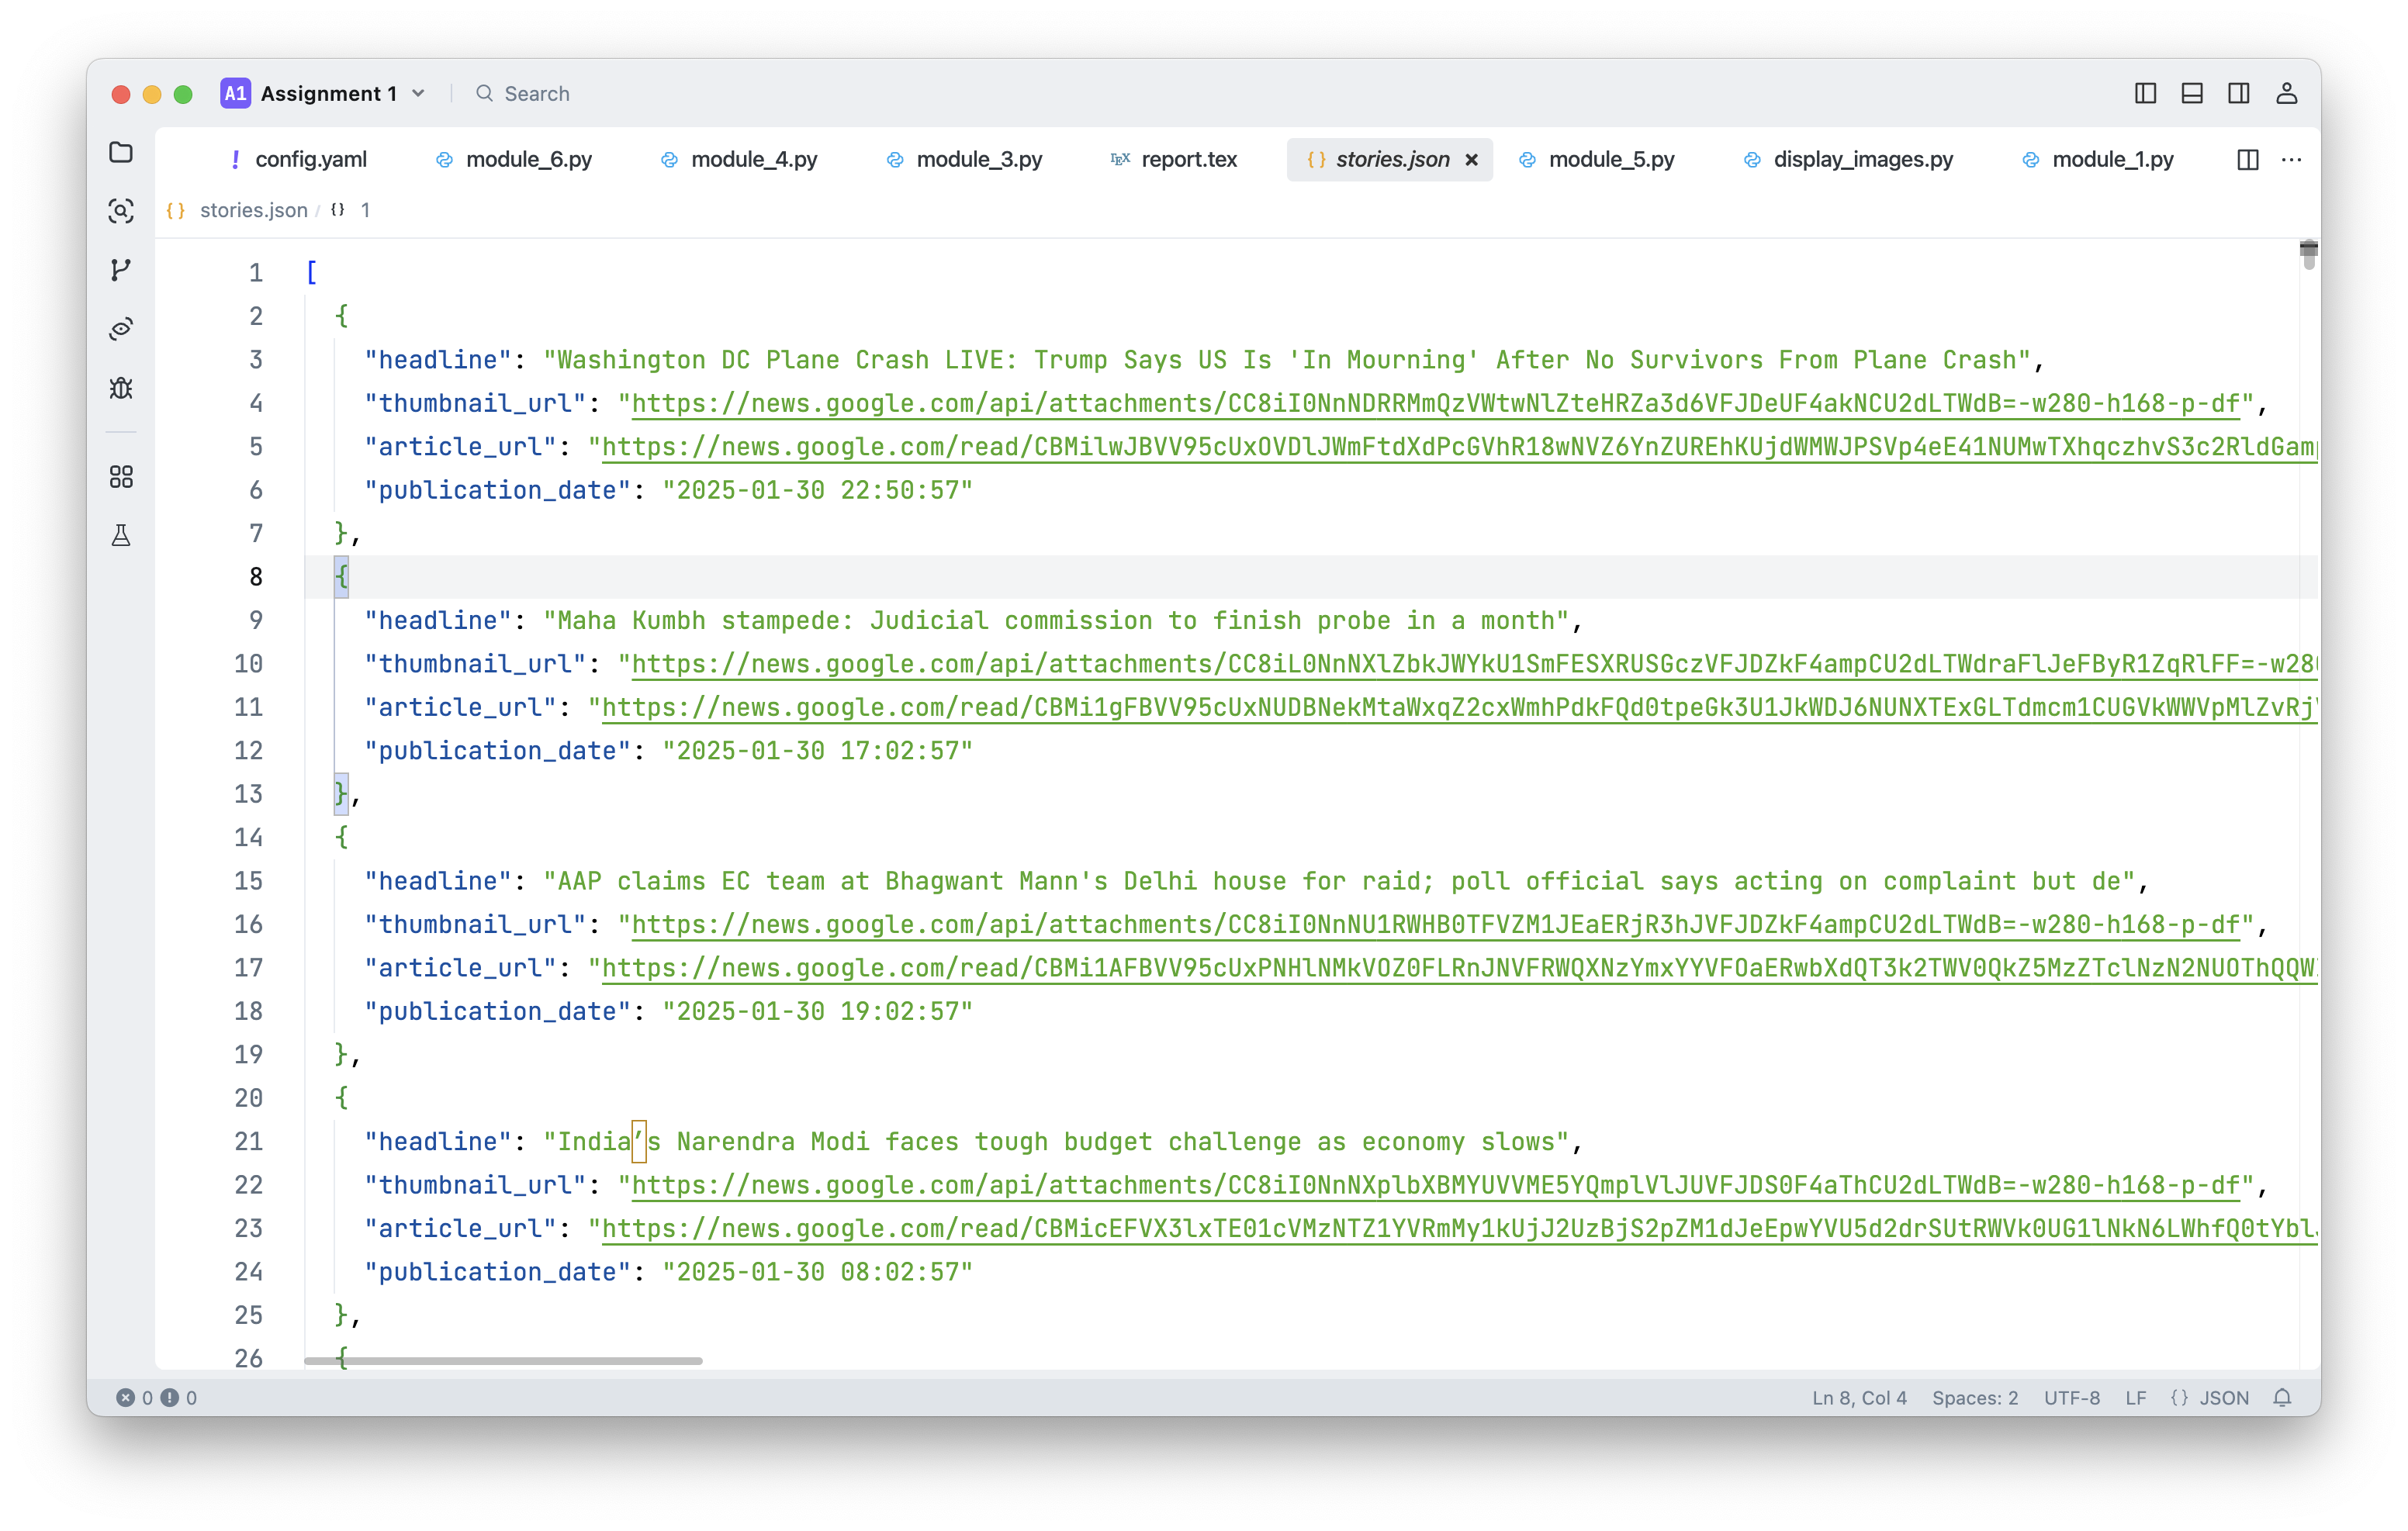
\includegraphics[width=\textwidth]{report/module_3 results_2.png}
    \caption{Results from Module 3 execution, stored as a json file}
    \label{fig:module3-results-2}
\end{figure}

\\

\subsection{Module 4: Database Operations}
This module manages all database interactions using a robust transaction-based approach. It handles both article metadata and binary image data storage, ensuring data integrity through proper error handling and rollback mechanisms. The module is designed to be resilient against common database errors and connection issues.
To run this module, execute the following command:
\begin{lstlisting}[language=bash]
python module_4.py 
\end{lstlisting}

\begin{lstlisting}[language=Python]
class NewsDatabase:
    def store_article(self, story):
        try:
            self.cursor.execute("""
                INSERT INTO news_articles 
                (headline, article_url, publication_date)
                VALUES (%s, %s, %s)
                RETURNING id
            """, (
                story['headline'],
                story['article_url'],
                story['publication_date']
            ))
            
            article_id = self.cursor.fetchone()[0]
            
            if story['thumbnail_url']:
                response = requests.get(story['thumbnail_url'])
                self.cursor.execute("""
                    INSERT INTO news_images 
                    (article_id, thumbnail_url, image_data)
                    VALUES (%s, %s, %s)
                """, (
                    article_id,
                    story['thumbnail_url'],
                    psycopg2.Binary(response.content)
                ))
            
            self.conn.commit()
            return True
            
        except Exception as e:
            self.conn.rollback()
            return False
\end{lstlisting}

\begin{figure}[H]
    \centering
    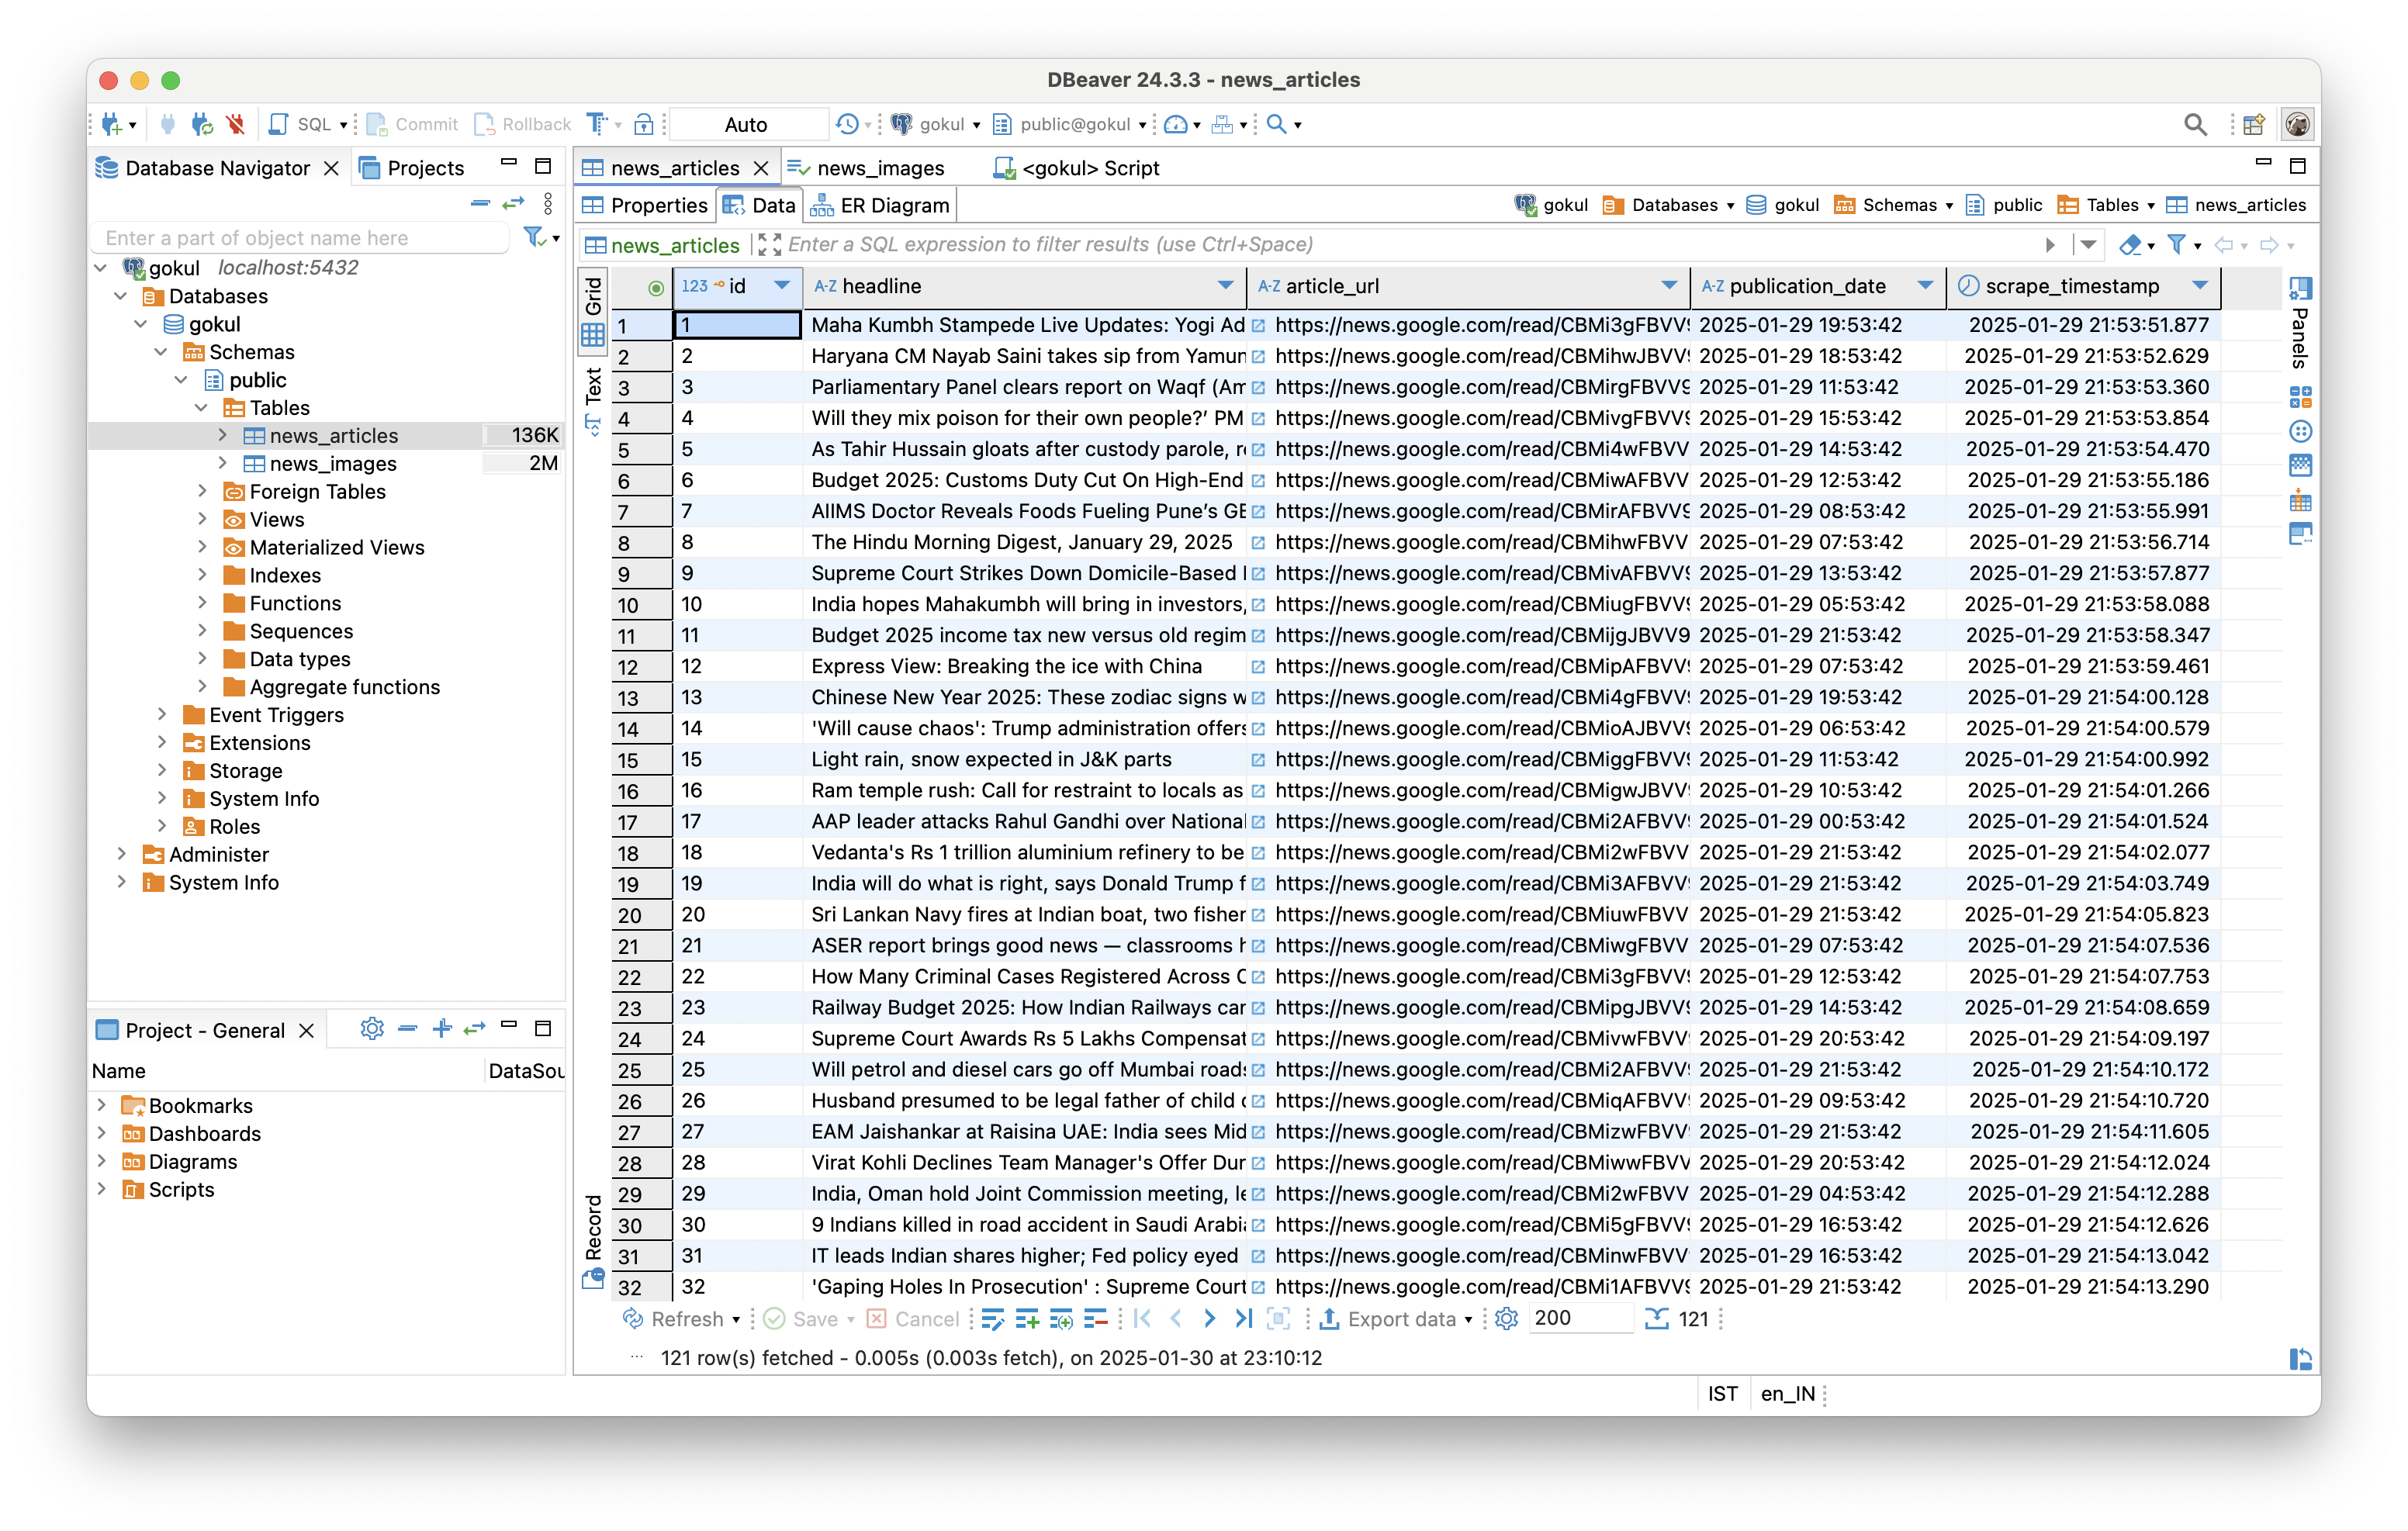
\includegraphics[width=\textwidth]{report/module_4 news_articles.png}
    \caption{Results from Module 4 execution on news articles table}
    \label{fig:module4-results-1}
\end{figure}

\begin{figure}[H]
    \centering
    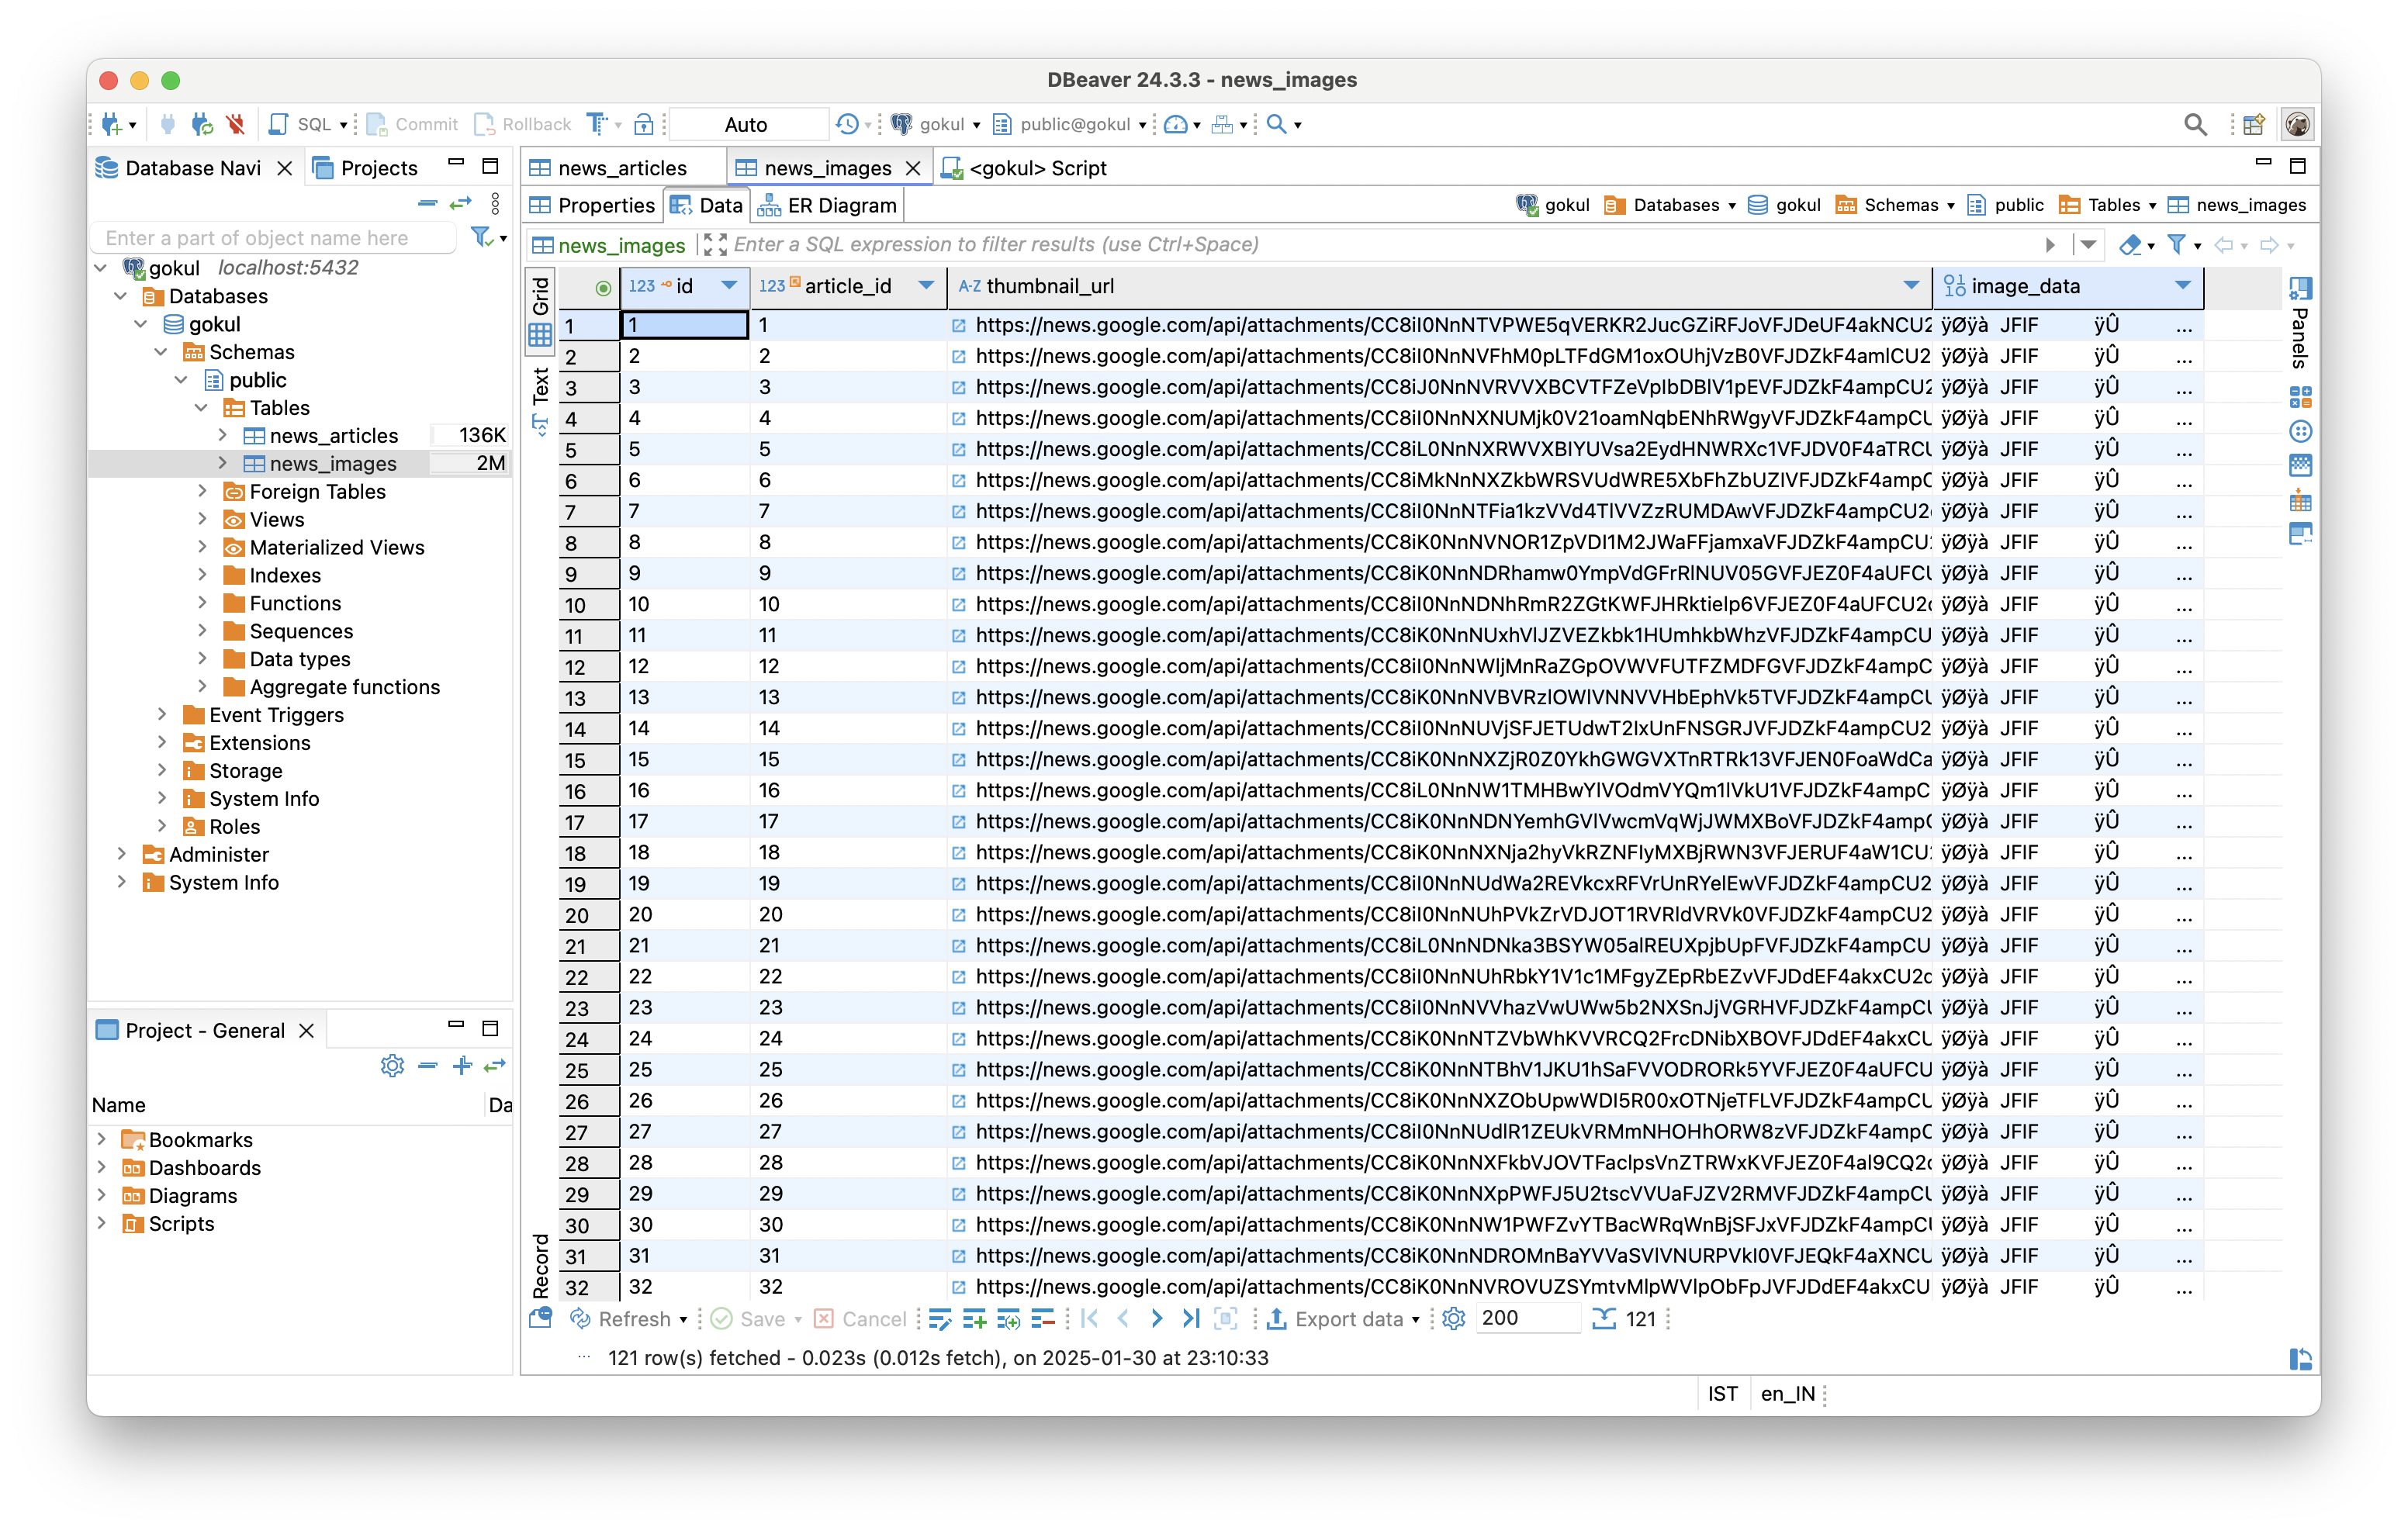
\includegraphics[width=\textwidth]{report/module_4 news_images.png}
    \caption{Results from Module 4 execution on news images table}
    \label{fig:module4-results-2}
\end{figure}

\\

\subsection{Module 5: Duplication Checker}
The Duplication Checker implements sophisticated article comparison logic using the SequenceMatcher algorithm. It prevents duplicate entries by comparing headlines with configurable similarity thresholds for same-day and different-day articles. The module optimizes database queries using appropriate indexes for efficient comparison operations.
This module employs a similarity threshold system based on publication timing. For articles published on the same day, a lower similarity threshold is used since similar breaking news stories often appear with slight variations. For articles published on different days, a higher threshold is applied to ensure only truly duplicate content is flagged. This dual-threshold approach helps balance between catching real duplicates while allowing legitimate similar same-day coverage.

To run this module, execute the following command:
\begin{lstlisting}[language=bash]
python module_5.py 
\end{lstlisting}

\begin{lstlisting}[language=Python]
class DuplicationChecker:
    def is_duplicate(self, story, same_day_threshold=0.9, 
                    different_day_threshold=0.95):
        story_date = story['publication_date'][:10]
        
        # Check same day articles
        self.cursor.execute("""
            SELECT headline, publication_date 
            FROM news_articles
            WHERE SUBSTRING(publication_date, 1, 10) = %s
        """, (story_date,))
        
        for existing_headline, _ in self.cursor.fetchall():
            similarity = self.calculate_headline_similarity(
                story['headline'], 
                existing_headline
            )
            if similarity >= same_day_threshold:
                return True, "Same day duplicate"
        
        return False, "No duplicate found"
\end{lstlisting}

\begin{figure}[H]
    \centering
    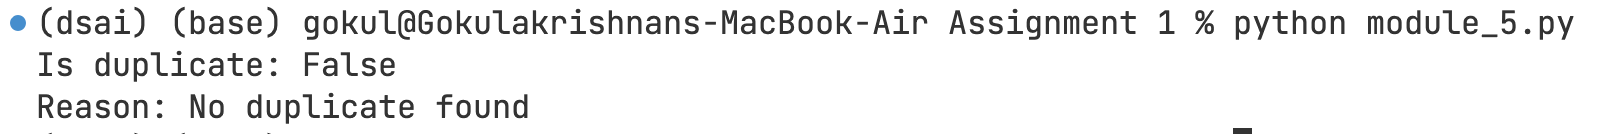
\includegraphics[width=\textwidth]{report/module_5.png}
    \caption{Results from Module 5 execution}
    \label{fig:module5-results}
\end{figure}

\\

\subsection{Module 6: Pipeline Orchestrator}
This module serves as the central coordinator for the entire pipeline, managing the execution flow and error handling. It implements configurable scheduling with sleep intervals and maintains comprehensive logging of all operations. The orchestrator ensures graceful handling of failures at any stage of the pipeline while maintaining continuous operation. You can change the frequency of the chron job by modifying the frequency variable in the config.yaml file.
To run this module, execute the following command:
\begin{lstlisting}[language=bash]
python module_6.py 
\end{lstlisting}

\begin{lstlisting}[language=Python]
def run_pipeline():
    setup_logging()
    
    with open('config.yaml', 'r') as f:
        config = yaml.safe_load(f)
    
    frequency = config.get('pipeline', {}).get('frequency', 3600)
    
    while True:
        try:
            # Execute pipeline steps
            home_scraper = NewsHomeScraper('config.yaml')
            homepage_content = home_scraper.scrape_homepage()
            
            if homepage_content:
                top_stories_scraper = TopStoriesScraper(
                    homepage_content, 
                    config
                )
                top_stories_url = (
                    top_stories_scraper.find_top_stories_link()
                )
                
                if top_stories_url:
                    story_extractor = StoryExtractor(config)
                    stories = story_extractor.extract_stories(
                        top_stories_url
                    )
                    
                    if stories:
                        db = NewsDatabase(config)
                        for story in stories:
                            db.store_article(story)
                        db.close()
            
            time.sleep(frequency)
            
        except Exception as e:
            logging.error(f"Pipeline failed: {str(e)}")
\end{lstlisting}

\begin{figure}[H]
    \centering
    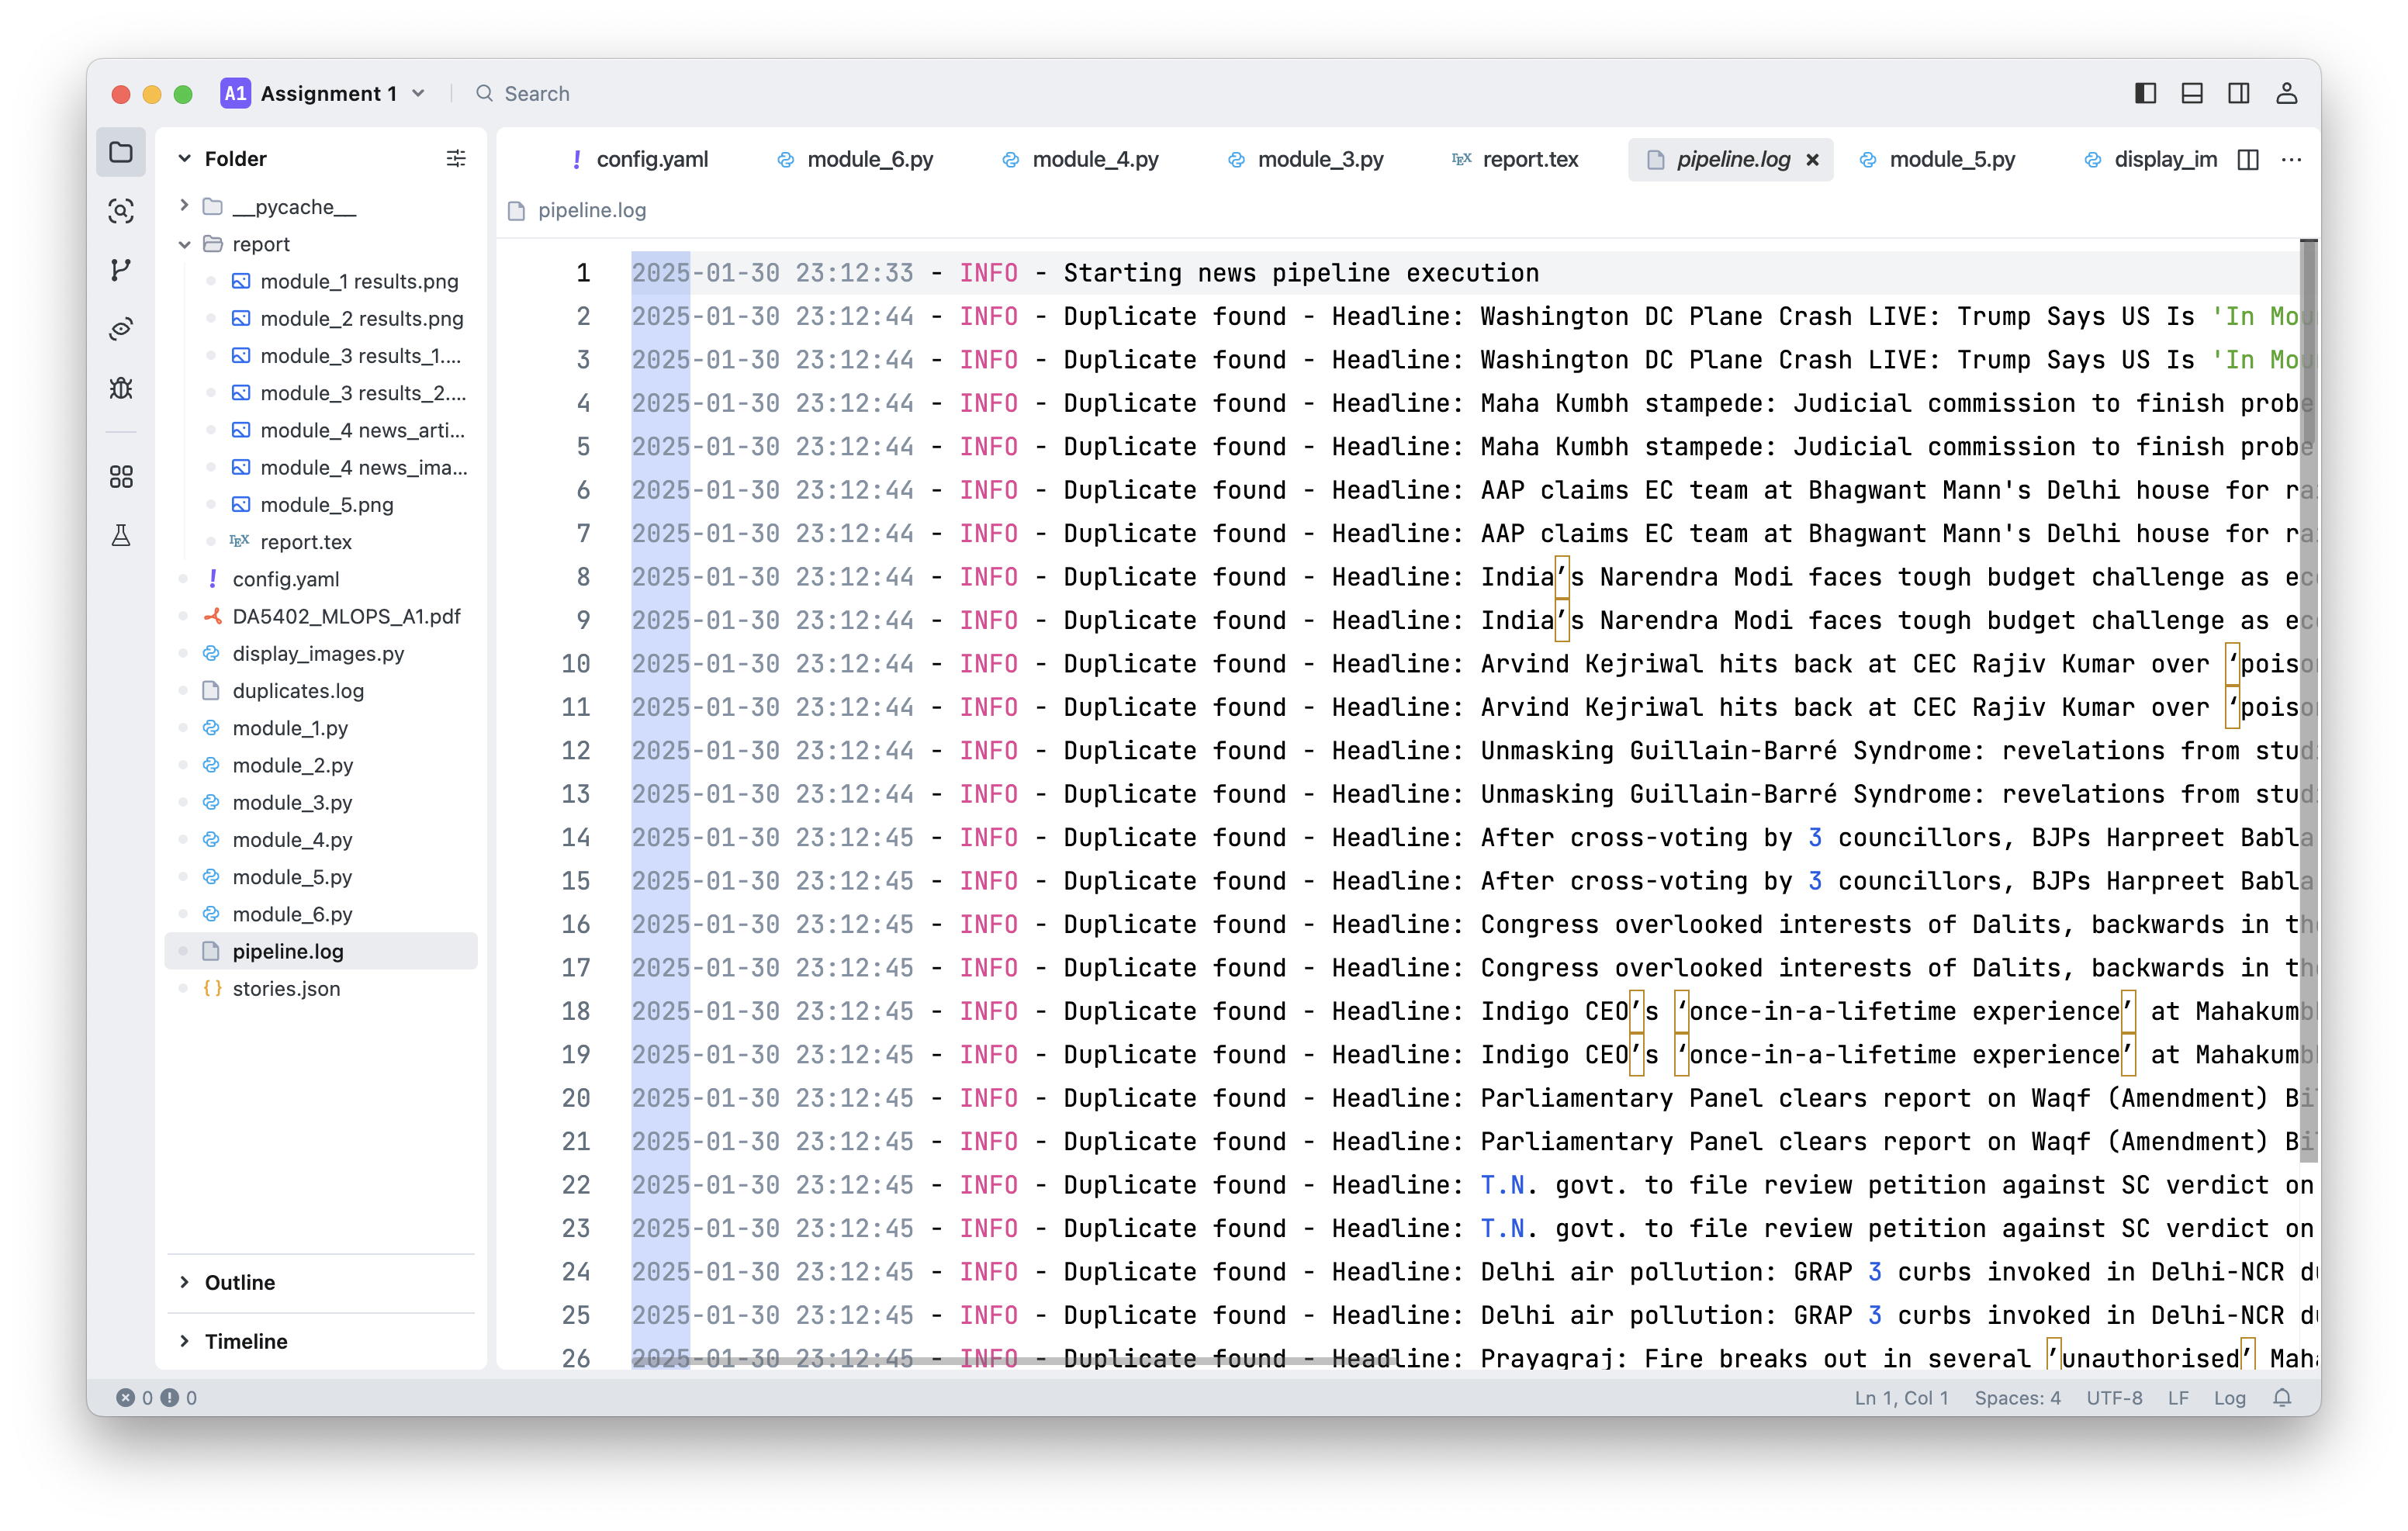
\includegraphics[width=\textwidth]{report/module_6.png}
    \caption{Results from Module 6 execution}
    \label{fig:module6-results}
\end{figure}


\section{Configuration}
The system uses a YAML configuration file:

\begin{lstlisting}[language=PYTHON]
# Base configuration for Google News Scraper
scraper:
  base_url: "https://news.google.com"
  user\_agent: "Mozilla/5.0 (Windows NT 10.0; Win64; x64) AppleWebKit/537.36"
  top\_stories\_pattern: "Top stories"

database:
  dbname: "gokul"
  user: "gokul"
  password: "****"
  host: "localhost"
  port: 5432

output:
  log\_file: "scraper.log"
  images\_folder: "images"

deduplication:
  methods: ["headline", "url", "content\_similarity"]
  similarity\_threshold: 0.85

pipeline:
  frequency: 3600  # Run every hour (in seconds)
\end{lstlisting}

\section{Logging}
The system maintains a log file:
\begin{itemize}
    \item pipeline.log: Records pipeline execution details
\end{itemize}

\section{Conclusion}
The implemented system successfully automates the process of:
\begin{itemize}
    \item Scraping news articles from Google News
    \item Detecting and preventing duplicate articles
    \item Storing articles and images in a PostgreSQL database
    \item Running continuously with configurable frequency
\end{itemize}

The modular design allows for easy maintenance and future enhancements.

\end{document}